Das asymmetrische Schlüssel Konzept geht auf das von Whitfield Diffie und Martin Hellmann im Jahr 1976 entwickelte Verschlüsselungsverfahren DH76 zurück. In dem Verfahren werden zwei voneinander abhängige Schlüssel generiert. Ein Schlüssel dient zur Verschlüsselung und ist geheim. Der andere Schlüssel wird zur Entschlüsselung verwendet und ist öffentlich. Die digitale Signatur dient vorrangig nicht der Unkenntlichmachung der Dokumente und Information, sondern der Feststellung, ob die signierten Informationen unversehrt bei dem Empfänger angekommen sind oder verändert wurden. Darüber hinaus zur Identifizierung des Signaturschlüssel-Inhabers. Die Prüfung auf Echtheit des Signaturschlüssels wird mit dem öffentlichen Schlüssel übernommen. Der private Schlüssel signiert nicht das gesamte Dokument, sondern nur einen repräsentativen Bereich. \cite{techno1}
\begin{figure}[!ht]
    \centering
    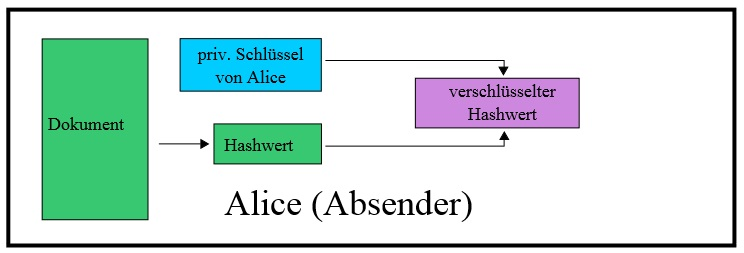
\includegraphics[width=\textwidth]{ErstellungAbsender2.jpg}
    \caption[Erstellung eines Dokuments mit digitaler Signatur]{\small{Erstellung eines Dokuments mit digitaler Signatur. \cite{techno3}}}
    \label{fig:2}
\end{figure}\\
Der erste Schritt im Signierungsprozess ist das bilden eines Fingerabdrucks (Hashwert) des Dokuments. Der Fingerabdruck wird mittels Hash-Algorithmus von einem Teil des Dokuments erstellt und ist mit hoher Wahrscheinlichkeit eindeutig. "'Ein Hash-Algorithmus ist eine mathematische Funktion, die eine beliebig große Menge an Eingabewerten möglichst gleichmäßig auf eine eingeschränkte Ausgabemenge abbildet"' \cite{techno2}. Eine absolute Eindeutigkeit des Fingerabdrucks kann auf Grund des Zufallsprinzips bei Hash-Algorithmen nicht gewährleistet werden. Anhand des Fingerabdrucks kann nicht auf das Dokument und deren Inhalt geschlossen werden. Weiterhin ist die Erstellung des Dokuments aus dem Fingerabdruck nicht möglich, da der Hashwert von einem beliebigen Teil des Dokuments erstellt wird. Im zweiten Schritt des Prozesses wird der Fingerabdruck mittels privaten Signaturschlüssels zur Sicherstellung der Unversehrtheit des Dokuments verschlüsselt. Im letzten Schritt werden der verschlüsselte Fingerabdruck und das Dokument zu einer Datei vereint. \cite{techno1}   